\documentclass[Berkeley]{beamer}

\usetheme{Copenhagen}

\usepackage{bm}
\usepackage{amsmath}
\usepackage{amssymb}
\usepackage{graphicx}
\usepackage{multimedia}
\AtBeginSection[]{
  \begin{frame}
  \vfill
  \centering
  \begin{beamercolorbox}[sep=8pt,center,shadow=true,rounded=true]{title}
    \usebeamerfont{title}\insertsectionhead\par%
  \end{beamercolorbox}
  \vfill
  \end{frame}
}


\title{Selective Harmonic Elimination as a optimal control problem}
\author{Jesús Oroya}
\institute{Chair of Computational Mathematics}
\begin{document}
    \maketitle
    \begin{frame}
        \frametitle{Índice}
        \tableofcontents    
    \end{frame}


    

\section{Selective Harmonic Elimination}
%%%%%%%%%%%%%%%%%%%%%%%%%%%%%%%%%%%%%%%%%%%%%
\begin{frame}
    \frametitle{Selective Harmonic Elimination}
    \framesubtitle{Elementos básicos}
    \begin{itemize}
        \item     Se considerará la función $f(\tau) \ | \ \tau \in [0,\pi]$ que solo puede tomar los valores $\{-1,1\}$.
        \item Consideraremos que esta función tiene simetría de media onda, es decir: $f(\tau) = -f(\tau + \pi)$.
    \end{itemize}

\end{frame}
%%%%%%%%%%%%%%%%%%%%%%%%%%%%%%%%%%%%%%%%%%%%%
\begin{frame}
    \frametitle{Selective Harmonic Elimination}
    \framesubtitle{Elementos básicos}
    \begin{itemize}
        \item De esta manera, los $f(\tau)$ se puede desarrollar en serie de Fourier como:
    \begin{gather}
        f(\tau ) = \sum_{i \in impar} a_i \cos(i\tau)+ \sum_{j \in impar}  b_j \sin(j \tau) 
    \end{gather}
    
    Donde $a_i$ y $b_j$  son:
    \begin{gather}
        a_i = \frac{2}{\pi} \int_0^\pi f(\tau ) \cos(i \tau)d\tau \ | \ \forall i \ impar \label{an}\\
        b_j = \frac{2}{\pi} \int_0^\pi f(\tau)  \sin(j \tau) d\tau \ | \ \forall j \ impar \label{bn}
    \end{gather}
    \end{itemize}

\end{frame}
%%%%%%%%%%%%%%%%%%%%%%%%%%%%%%%%%%%%%%%%%%%%%
\begin{frame}
    
    \frametitle{Definición del Problema SHE}

    \begin{problem}[SHE para dos niveles]
        \begin{itemize}
            \item Consideramos dos conjuntos de números impares $\mathcal{E}_a$ y $\mathcal{E}_b$ con cardinalidades $|\mathcal{E}_a| = N_a$ y  $|\mathcal{E}_b| = N_b$ respectivamente.
            \item Consideramos los vectores objetivo $\bm{a}_T  \in \mathbb{R}^{N_a}$ y $\bm{b}_T  \in \mathbb{R}^{N_b}$.
            \item  Buscamos una función  $f(\tau )  \in \{-1,1\} \ | \  \forall  \tau \in (0,\pi)$  cuyos coeficientes de Fourier satisfagan: 
            \begin{gather}
                \begin{cases}
                    a_i = (\bm{a}_T)_i & \forall i \in \mathcal{E}_a \\
                    b_j = (\bm{b}_T)_j & \forall \ j \in \mathcal{E}_b
                \end{cases}
            \end{gather}

        \end{itemize}
    \end{problem}
\end{frame}
%%%%%%%%%%%%%%%%%%%%%%%%%%%%%%%%%%%%%%%%%%%%%

\begin{frame}
    \frametitle{Optimización de ángulos de conmutación}
    Si denotamos ángulos de conmutación como 
    \begin{gather}
        \bm{\phi} = [\phi_1,\phi_2,\dots,\phi_M] \in \mathbb{R}^M 
    \end{gather}
    podemos escribir los coeficientes de Fourier (\ref{an}) y (\ref{bn}) en función de $\bm{\phi}$ como: 
    \begin{align}
        a_i(\bm{\phi})  = & +\frac{4}{i\pi} \sum_{k=1}^{M} (-1)^{k+1}\sin(i\phi)  & \ | \ \forall i \in \mathcal{E}_a \\
        b_j(\bm{\phi})  = & - \frac{2}{j\pi  } \bigg[ 1  + (-1)^{M}+ 2\sum_{k=1}^M  (-1)^{k+1}\cos(j\phi_k) \bigg] & \ | \ \forall j \in \mathcal{E}_b
    \end{align}
\end{frame}

%%%%%%%%%%%%%%%%%%%%%%%%%%%%%%%%%%%%%%%%%%%%%%%%%%%

\begin{frame}
    \frametitle{}
    \begin{problem}
        \begin{itemize}
            \item Consideramos dos conjuntos de números impares $\mathcal{E}_a$ y $\mathcal{E}_b$ con cardinalidades $|\mathcal{E}_a| = N_a$ y  $|\mathcal{E}_b| = N_b$.
            \item Consideramos los vectores $\bm{a}_T  \in \mathbb{R}^{N_a}$ y $\bm{b}_T  \in \mathbb{R}^{N_b}$
            \item Consideramos un número de conmutaciones $M$
            \item Buscamos los ángulos de conmutación $\bm{\phi} \in \mathbb{R}^M$ mediante el problema de minimización:
        \begin{gather}
            \min_{\bm{\phi} \in \mathbb{R}^M} \Big[
            \sum_{i \in \mathcal{E}_a} (a_i(\bm{\phi}) - a^i_T)^2 + 
            \sum_{j \in \mathcal{E}_b} (b_j(\bm{\phi}) - b^j_T)^2  
            \Big] \\
            \notag \text{sujeto a:} \\ 
            \notag    0 < \phi_1  < \phi_2 < \dots  < \phi_k < \dots < \phi_{M-1}  <   \phi_{M} < \pi
            \label{constraints}
        \end{gather} 
    \end{itemize}
\end{problem}

\end{frame}



    \section{Coeficientes de Fourier como sistemas dinámicos}
\begin{frame}
    \frametitle{Coeficientes de Fourier como sistemas dinámicos}
    \begin{itemize}
        \item Mediante el teorema fundamental de cálculo transformarmos la integrales en ecuaciones diferenciales, de la siguiente manera:
    \end{itemize}
    \begin{gather}
        \alpha_i(\tau) = \frac{2}{\pi}\int_0^\tau f(\tau) \sin(i\tau)d\tau 
        \Rightarrow
        \begin{cases} \label{ode}
            \dot{\alpha_i}(\tau) & = \frac{2}{\pi}f(\tau)\sin(i\tau) \\  
            \alpha_i(0) & = 0       
        \end{cases}
    \end{gather}
    
    \begin{gather}
        \beta_j(\tau) = \frac{2}{\pi}\int_0^\tau f(\tau) \cos(j\tau)d\tau 
        \Rightarrow
        \begin{cases} \label{ode}
            \dot{\beta}_j(\tau) & = \frac{2}{\pi}f(\tau)\cos(j\tau) \\  
            \beta_j(0) & = 0       
        \end{cases}
    \end{gather}

\end{frame}
%%%%%%%%%%%%%%%%%%%%%%%%%%%%%%%%%%%%%%%%%%%%%%%
\begin{frame}
    \frametitle{Coeficientes de Fourier como sistemas dinámicos}
    
    \begin{itemize}
        \item De esta manera, el estado $\{ \alpha_{i},\beta_{j} \}$ en el intante de tiempo $\tau = \pi$ son los coeficientes de Fourier de $f(\tau) $
    \end{itemize}
    \begin{gather}
        \begin{cases} \label{ode}
            \dot{\alpha_i}(\tau) & = \frac{2}{\pi}f(\tau)\sin(i\tau) \\  
            \alpha_i(0) & = 0       
        \end{cases}
        \Rightarrow 
        \alpha_i(\pi) = a_i^T
    \end{gather}
    
    \begin{gather}
        \begin{cases} 
            \dot{\beta}_j(\tau) & = \frac{2}{\pi}f(\tau)\cos(j\tau) \\  
            \beta_j(0) & = 0       
        \end{cases}
        \Rightarrow 
        \beta_i(\pi) = b_i^T
    \end{gather}
    Entonces el problema se traduce a encontrar un control $f(t)$ que conduzca al sistema desde el origen de coordenadas hasta el punto objetivo marcado.
\end{frame}
%%%%%%%%%%%%%%%%%%%%%%%%%%%%%%%%%%%%%%%%%%%%%%%
\begin{frame}
    \frametitle{Coeficientes de Fourier como sistemas dinámicos}
    
    \begin{itemize}
        \item Consideramos los conjuntos $\mathcal{E}_a = {1}$ y $\mathcal{E}_b = {1}$
        \item El sistema dinámico se escribe como:
        \begin{gather}
            \begin{cases} 
                \dot{\alpha}_1(\tau) & = \frac{2}{\pi}f(\tau)\sin(\tau) \ | \  \alpha(0) = 0\\
                \dot{\beta}_1(\tau) & = \frac{2}{\pi}f(\tau)\cos(\tau)  \ | \  \beta(0) = 0
            \end{cases}  
        \end{gather}

        \item Si aplicamos $f(\tau)$ al sistema $(\alpha_1(\tau),\beta_1(\tau))$, entonces el vector de estado final 
        \begin{gather}
            (\alpha_1(\pi),\beta_1(\pi)) = (a_1,b_1) \text{ de } f(\tau)
        \end{gather}
    \end{itemize}
\end{frame}

\begin{frame}
    \frametitle{Coeficientes de Fourier como sistemas dinámicos}
    \begin{figure}
        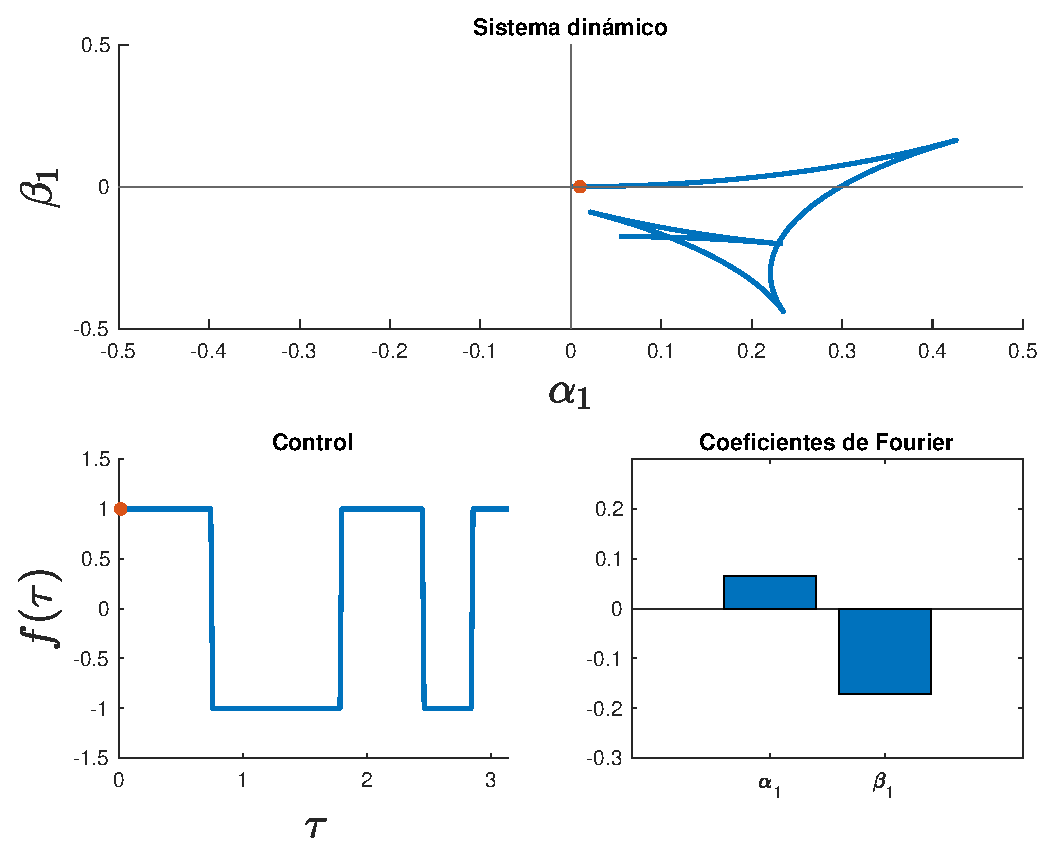
\includegraphics[scale=0.4]{imgs/S0001.eps}
        \caption{Evolución de un sistema $\{\alpha_1,\beta_1\}$ Sistema dinámico}
    \end{figure}
\end{frame}


%%%%%%%%%%%%%%%%%%%%%%%%%%%%%%%%%%%%%%%%%%%%%%%

    \section{Formulación como problema de control}
\begin{frame}
    \frametitle{Problema de Control}
    \begin{problem}[OCP para SHE de dos niveles]\label{OCP1}
        \begin{itemize}
            \item Consideramos dos conjuntos de números impares $\mathcal{E}_a$ and $\mathcal{E}_b$ con cardinalidades $|\mathcal{E}_a| = N_a$ y  $|\mathcal{E}_b| = N_b$.
            \item Consideramos los vectores objetivos $\bm{a}_T  \in \mathbb{R}^{N_a}$ y $\bm{b}_T  \in \mathbb{R}^{N_b}$.
            \item Buscamos la función  $f(\tau ) \ | \ \tau \in (0,\pi)$ que minimiza el siguiente funcional de coste:

        \end{itemize}
            \begin{gather}
            J[f(\tau)] =  \| \bm{a}_T - \bm{\alpha}(T)\|^2 + \| \bm{b}_T - \bm{\beta}(T)\|^2 
            + \epsilon \int_0^{\pi} \mathcal{L}(f) d\tau  
        \end{gather}
    \end{problem}
\end{frame}

\begin{frame}
    \frametitle{}
    \begin{problem}[OCP para SHE de dos niveles]
    De esta forma podemos escribir el siguiente problema de control óptimo:
    \begin{gather}
        \min_{|f(\tau) |<1} J[f(\tau)] \\
        \notag \text{suject to: } \\
        \notag \forall i \in \mathcal{E}_a\ \ 
        \begin{cases}
            \dot{\alpha}_i(\tau) = (2/\pi) \cos(i\tau) f(\tau) & \tau \in [0,\pi]\label{dyn}\\
            \alpha_i(0) = 0
        \end{cases} \\
        \notag \forall j \in \mathcal{E}_b\ \ 
        \begin{cases}
            \dot{\beta}_j(\tau) = (2/\pi) \sin(j\tau) f(\tau) & \tau \in [0,\pi]\label{dyn}\\
            \beta_j(0) = 0
        \end{cases} \\
    \end{gather}
    \end{problem}
\end{frame}



\begin{frame}
    \frametitle{Condiciones de optimalidad}

    Es necesario construir la función Hamiltoniana:
    \begin{gather}\label{hamil}
        H(f,\bm{p}^\alpha,\bm{p}^\beta,\tau) = \epsilon \mathcal{L}(f) + 
        G(\bm{p}^\alpha,\bm{p}^\beta,\tau) f
    \end{gather}
    Donde  hemos llamado $G(\bm{p}^\alpha,\bm{p}^\beta,\tau)$ a:
    \begin{gather}
        G(\bm{p}^\alpha,\bm{p}^\beta,\tau) = \frac{2}{\pi} \Bigg[ 
            \sum_{i \in \mathcal{E}_a} p^\alpha_i \cos(i\tau)+ 
            \sum_{j \in \mathcal{E}_b} p^\beta_j \sin(j\tau) 
        \Bigg]
    \end{gather}
    Y donde $\bm{p}^\alpha$ y $\bm{p}^\beta$ son los co-estados del sistema.
\end{frame}


\begin{frame}
    \frametitle{Principio de mínimo de Pontryagin}
    Cuando evaluamos el Hamiltoniano en los co-estados óptimos $\bm{p}_*^\alpha$ y $\bm{p}_*^\beta$ podemos encontrar la forma del control minimizando el Hamiltoniano.
    \begin{gather}\label{minH}
        H(\tau,\bm{p}_*^\alpha,\bm{p}^\beta_*,f_*) \leq
        H(\tau,\bm{p}_*^\alpha,\bm{p}^\beta_*,f)
    \end{gather}
    Entonces anilizaremos el problema 
    \begin{gather}
        \min_{|f|<1} H_*(f)
    \end{gather}
    Donde hemos llamado $H_*(f)$ a $H(\tau,\bm{p}_*^\alpha,\bm{p}^\beta_*,f)$
\end{frame}


\begin{frame}
    \frametitle{Condiciones necesarias de optimalidad}
    Entonces las condiciones necesarias de optimialidad para este problema se puede escribir como:
    \begin{gather}\label{hamil}
        H_*(f) = \epsilon \mathcal{L}(f) + 
        G(\bm{p}^\alpha_*,\bm{p}^\beta_*,\tau) f \\
        \frac{dH_*(f)}{df} = 0 \\
        \frac{dH_*^2(f)}{df^2} \geq 0 
    \end{gather}

\end{frame}

\begin{frame}
    \frametitle{Condiciones necesarias de optimalidad}
    Entonces las condiciones necesarias de optimialidad para este problema se puede escribir como:
    \begin{align}\label{hamil}
        H_*(f) = & \epsilon \mathcal{L}(f) + 
        G(\bm{p}^\alpha_*,\bm{p}^\beta_*,\tau) f \\
        \frac{dH_*(f)}{df} =  & \epsilon\frac{d\mathcal{L}}{df} + G(\bm{p}^\alpha_*,\bm{p}^\beta_*,\tau) = 0\\
        \frac{dH_*^2(f)}{df^2} = &  \epsilon \frac{d\mathcal{L}^2}{df^2}\geq 0 
    \end{align}

\end{frame}

\begin{frame}
    \frametitle{}
    \begin{figure}
        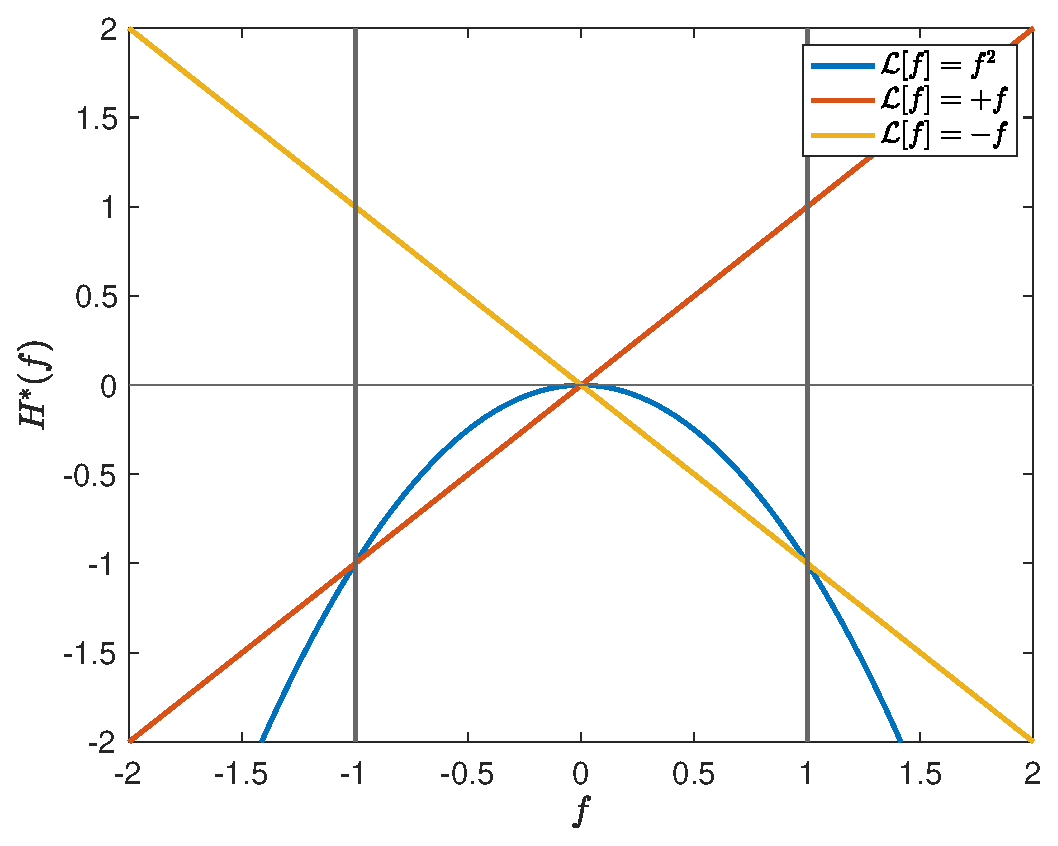
\includegraphics[scale=0.45]{imgs/bang-bang.eps}
    \end{figure}
\end{frame}

    \section{Experimentos numéricos}
\begin{frame}
    \frametitle{Caso para dos niveles}
    \begin{itemize}
        \item Para este ejemplo consideramos el siguiente conjunto de números impares: $\mathcal{E}_a = \{\emptyset\}$ y $\mathcal{E}_b = \{1,5,7,11,13\}$.
        \item Además consideramos el vector objetivo $\bm{b}_T = [m_a,0,0,0,0]$, donde  $m_a \in [0,1]$ es un parámetro.
        \item Compararemos la solución obenida mediante control óptimo con soluciones obtenidas en el problema con número de ángulos prefijados.
        \item Compararemos con las siguientes  penalizaciones: $\mathcal{L}(f) = -f$, $\mathcal{L}(f) = +f$ y $\mathcal{L}(f) = -f^2$
    \end{itemize}
\end{frame}

\begin{frame}
    \frametitle{Caso para dos niveles}
    \begin{figure}
        \centering
        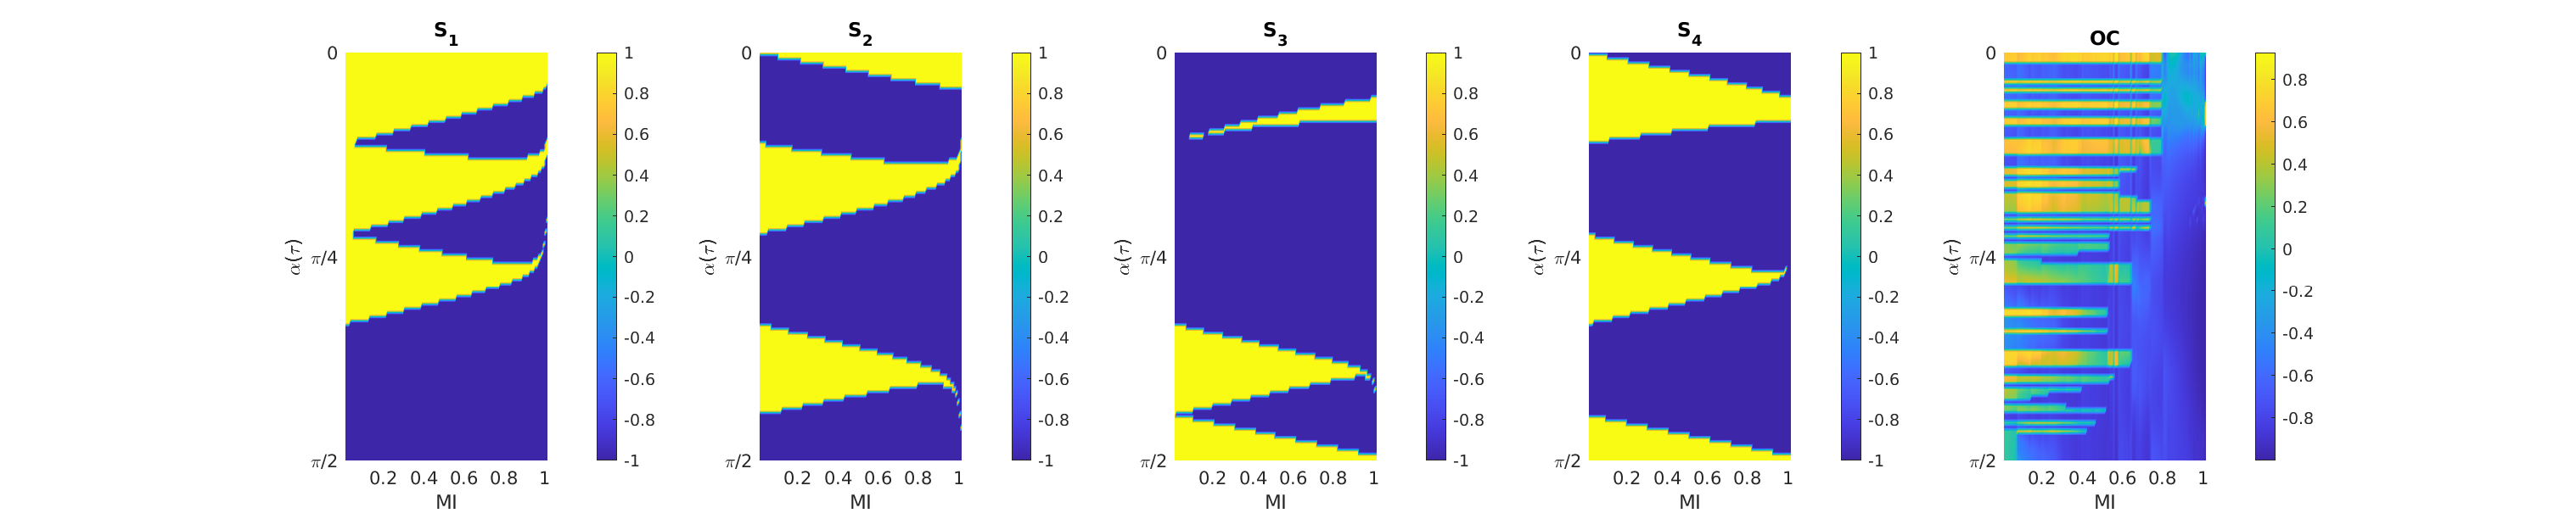
\includegraphics[scale=0.35]{../D0002-FullReport/img/EX01_surf.eps}
    \end{figure}
    
\end{frame}

\begin{frame}
    \frametitle{Caso para tres niveles}
    \begin{itemize}
        \item Podemos ver que en el caso en el que el control $f(\tau)$ solo pueda tomar valores entre $[0,1]$ obtenemos señales que pueden tomar tres niveles en el intervalo $[0,2\pi]$ gracias a la simetría de media de onda.
        \item Si resolvemos el problema de control óptimo pero esta vez cambiando las restricciones $|f(\tau)|<1$ por $\{0<f(\tau)<1\}$.
        \item Se ha realizado el mismo procedimiento que en el caso anterior.
    
    \end{itemize}

\end{frame}
\begin{frame}
    \frametitle{Caso para tres niveles}
    \begin{figure}
        \centering
        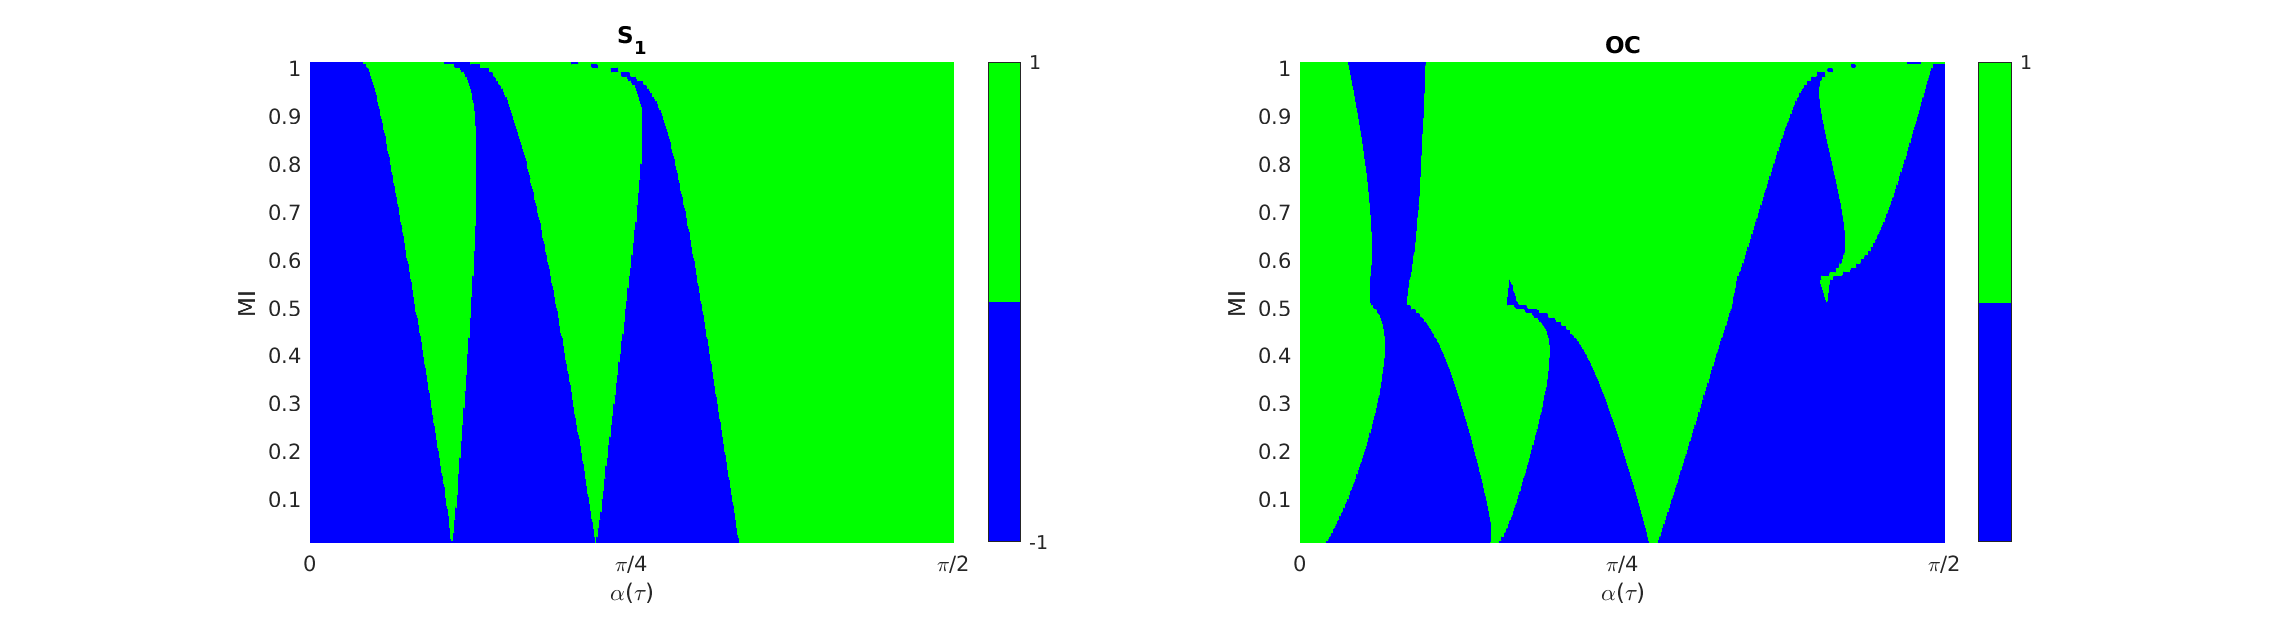
\includegraphics[scale=0.325]{../D0002-FullReport/img/EX01_surf_3LVL.eps}
    \end{figure}
    
\end{frame}



\end{document}